%----------------------------------------------------------------------------------------
%	PACKAGES AND OTHER DOCUMENT CONFIGURATIONS
%----------------------------------------------------------------------------------------

\documentclass[11pt]{diazessay} % Font size (can be 10pt, 11pt or 12pt)
\usepackage{float}
\usepackage{sectsty}
\usepackage[numbers]{natbib}
\sectionfont{\centering}
\usepackage{listings}
\usepackage{color}

\definecolor{dkgreen}{rgb}{0,0.6,0}
\definecolor{gray}{rgb}{0.5,0.5,0.5}
\definecolor{mauve}{rgb}{0.58,0,0.82}

\lstset{frame=tb,
  language=php,
  aboveskip=3mm,
  belowskip=3mm,
  showstringspaces=false,
  columns=flexible,
  basicstyle={\small\ttfamily},
  numbers=none,
  numberstyle=\tiny\color{gray},
  keywordstyle=\color{blue},
  commentstyle=\color{dkgreen},
  stringstyle=\color{mauve},
  breaklines=true,
  breakatwhitespace=true,
  tabsize=3
}
%----------------------------------------------------------------------------------------
%	TITLE SECTION
%----------------------------------------------------------------------------------------

\title{\textbf{Traffic Analysis} \\ {\Large\itshape A write-up}} % Title and subtitle

\author{\textbf{Matthew Doherty} \\ \textit{Rhodes University}} % Author and institution

\date{\today} % Date, use \date{} for no date

%----------------------------------------------------------------------------------------

\begin{document}

\maketitle % Print the title section

%----------------------------------------------------------------------------------------
%	ABSTRACT AND KEYWORDS
%----------------------------------------------------------------------------------------

%\renewcommand{\abstractname}{Summary} % Uncomment to change the name of the abstract to something else

\renewcommand{\thesection}{\arabic{section}}
\renewcommand{\thesubsection}{\arabic{subsection}}
\renewcommand{\thesubsubsection}{\arabic{subsubsection}}
\renewcommand{\thesubsection}{\thesection.\arabic{subsection}}
\renewcommand{\thesubsubsection}{\thesubsection.\arabic{subsubsection}}

\vspace{30pt} % Vertical whitespace between the abstract and first section

%----------------------------------------------------------------------------------------
%	ESSAY BODY
%----------------------------------------------------------------------------------------

% "*" means no numbering -> \section*{Introduction}

\section{Introduction}



%------------------------------------------------

\section{Traffic Overview}

\begin{figure}[H]
        \centering
        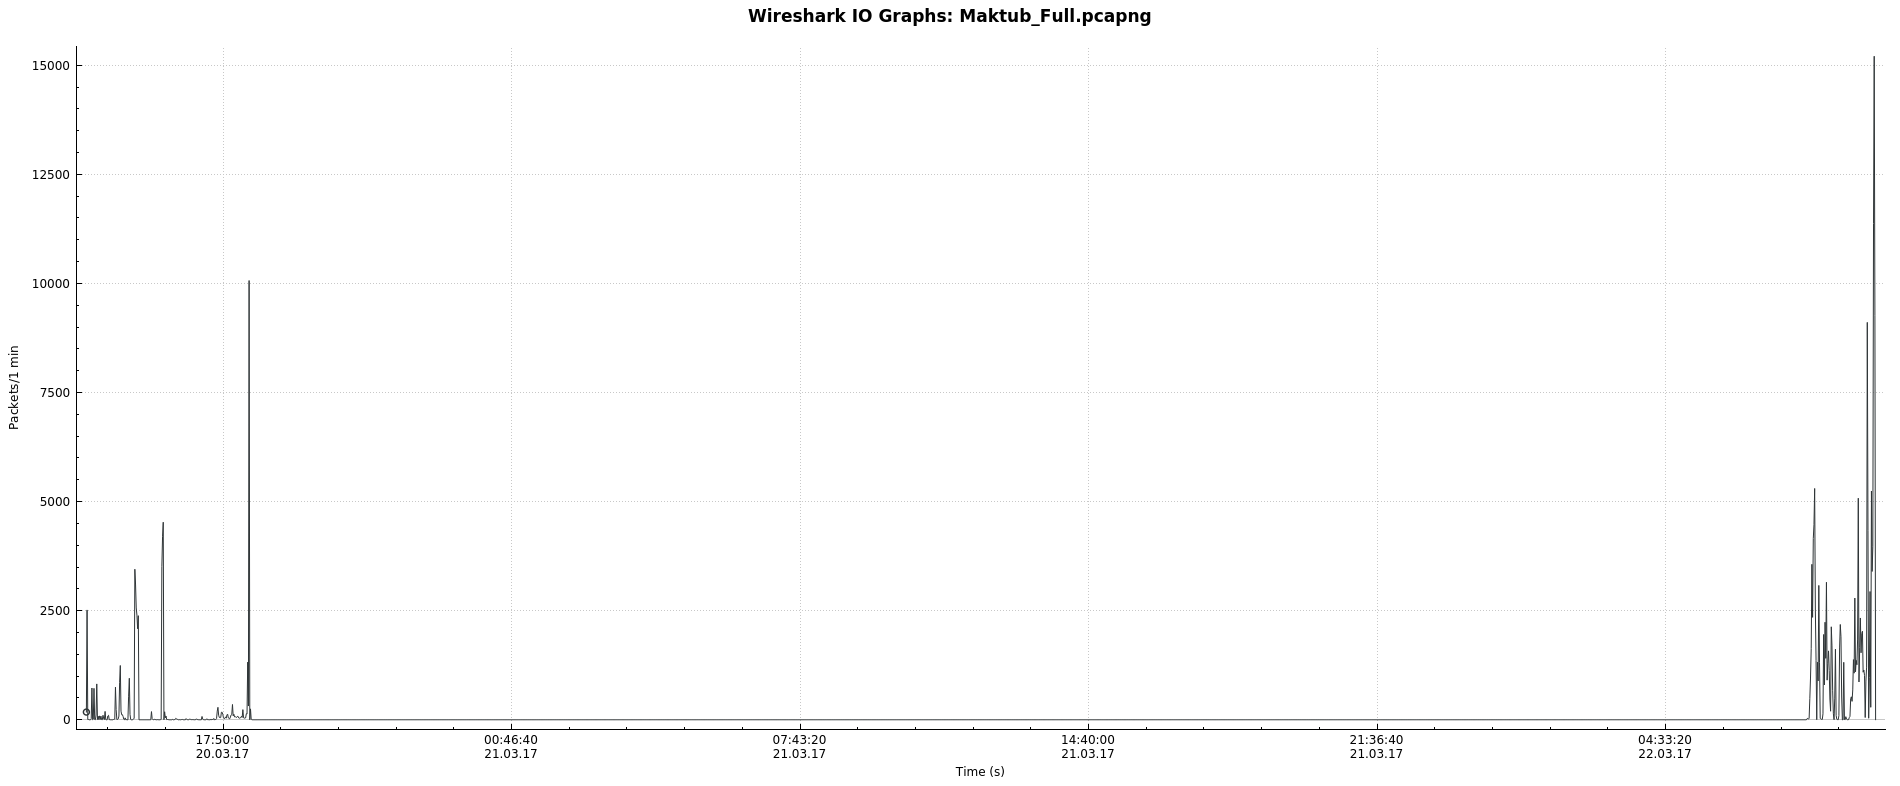
\includegraphics[scale=0.30]{Maktub_Full.png}
    \caption{Pcap Lifetime graph}
\end{figure}

\begin{figure}[H]
        \centering
        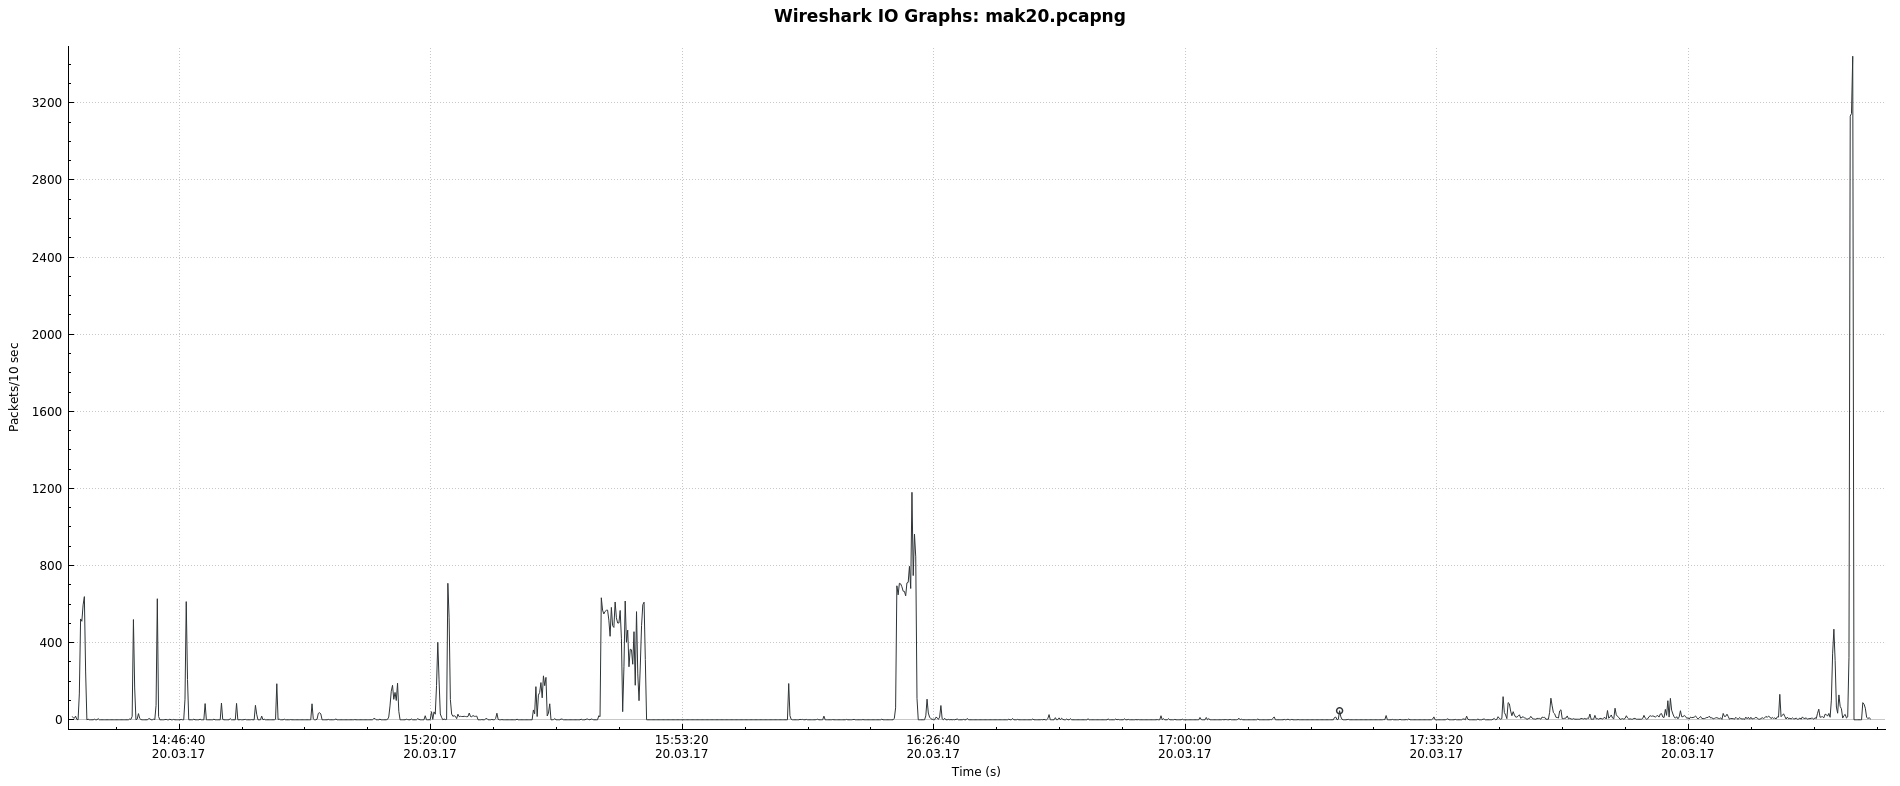
\includegraphics[scale=0.30]{mak20.png}
    \caption{IO graph for 2017-03-20} 
\end{figure}

\begin{figure}[H]
        \centering
        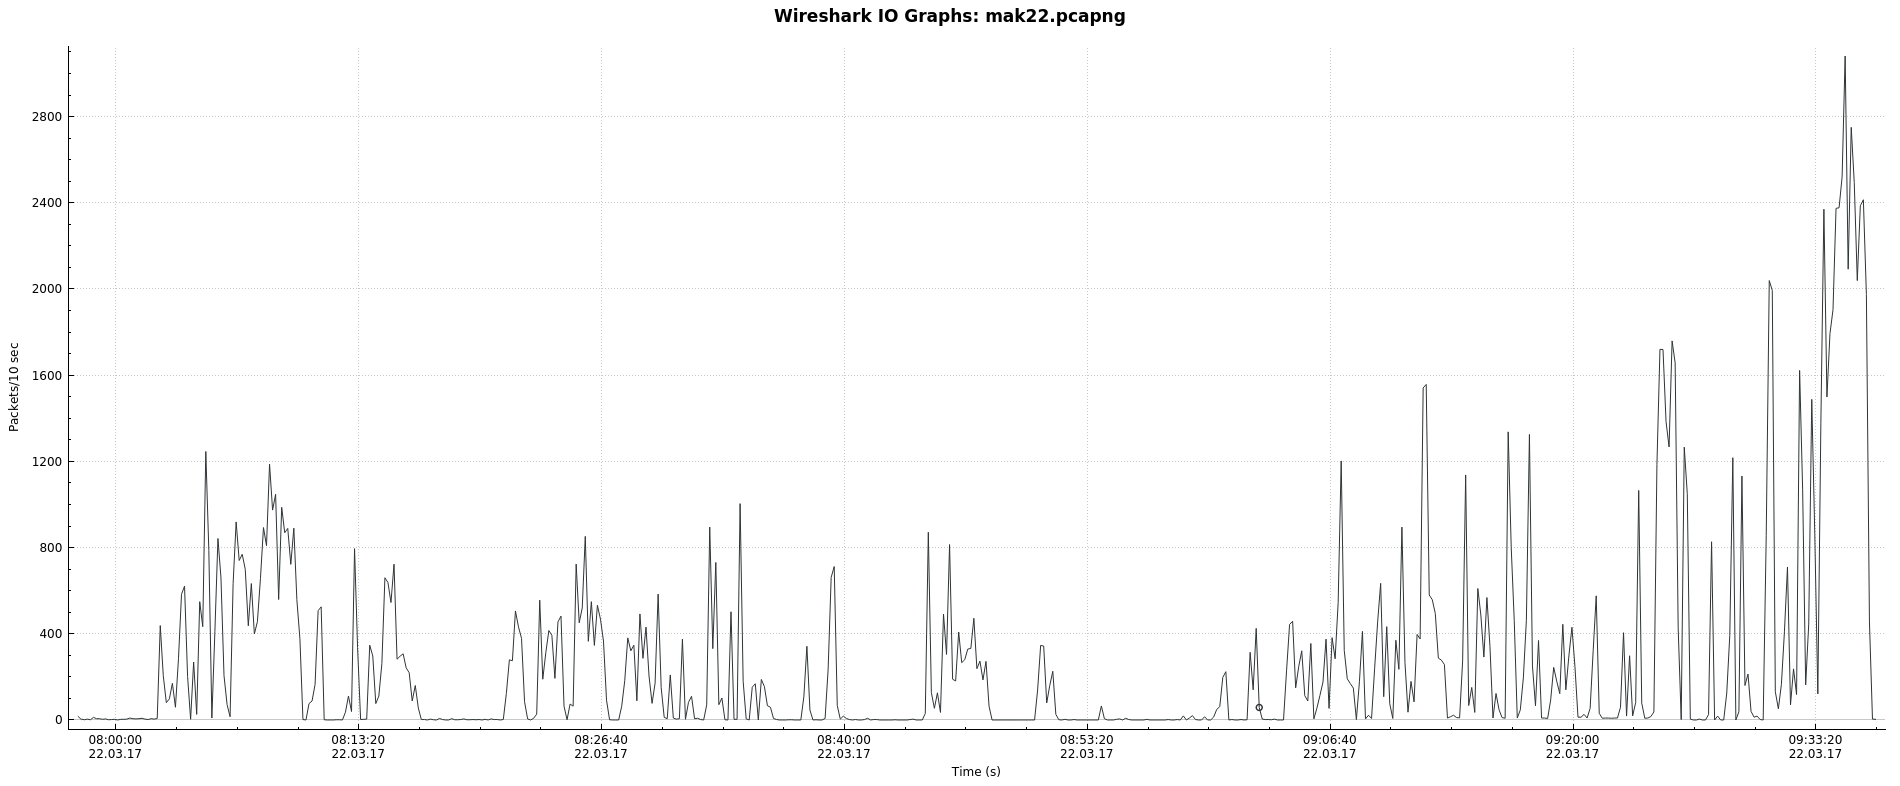
\includegraphics[scale=0.30]{mak22.png}
    \caption{IO Graph for 2017-03-22}
\end{figure}

Legitmate windows update from Ikai CDN 
DNS for onion domain singapoor 
DNS for cryptostorm to establish VPN Germany
Get Windows-CryptoAPI from comodoca 
China DNS req  for 1.83.255.178 

Cryptostorm VPN connect over TLS 
192.36.27.5 -> Amsterdam IP for onion (Entry node)

%------------------------------------------------

\section{Firewall Rules}

%------------------------------------------------

\section{Conclusion}

%----------------------------------------------------------------------------------------
%	BIBLIOGRAPHY
%----------------------------------------------------------------------------------------

\clearpage
%\bibliographystyle{unsrt}
\bibliographystyle{plainnat}
%plainnat, unsrtnat and abbrevnat)
\bibliography{sample.bib}

%----------------------------------------------------------------------------------------

\end{document}
